\documentclass[a4paper,12px]{article}
\usepackage{graphicx}
\usepackage[english]{babel}
\usepackage{fancyhdr}
\usepackage{lastpage}
\usepackage{xifthen}
\usepackage[linesnumberedhidden, titlenotnumbered]{algorithm2e}
\usepackage{lipsum}
\usepackage{hyperref}
\usepackage{array}
\usepackage{tabularx}

\usepackage{minted}
\usepackage{caption}
\usepackage{amssymb}

\pagestyle{fancy}
\lhead{
\includegraphics[width=7cm]{logoUvA}}
\rhead{\footnotesize \textsc {Report\\ \opdracht}}
\lfoot
{
    \footnotesize \studentA
    \ifthenelse{\isundefined{\studentB}}{}{\\ \studentB}
    \ifthenelse{\isundefined{\studentC}}{}{\\ \studentC}
    \ifthenelse{\isundefined{\studentD}}{}{\\ \studentD}
    \ifthenelse{\isundefined{\studentE}}{}{\\ \studentE}
}
\cfoot{}
\rfoot{\small \textsc {Page \thepage\ of \pageref{LastPage}}}
\renewcommand{\footrulewidth}{0.5pt}

\fancypagestyle{firststyle}
{
    \fancyhf{}
    \renewcommand{\headrulewidth}{0pt}
    \chead{
\includegraphics[width=7cm]{logoUvA}}
    \rfoot{\small \textsc {Page \thepage\ of \pageref{LastPage}}}
}

\setlength{\topmargin}{-0.3in}
\setlength{\textheight}{630pt}
\setlength{\headsep}{40pt}

% =================================== DOC INFO ===================================

\newcommand{\titel}{OpenMP}
\newcommand{\opdracht}{Assignment 2.3: Matrices}
\newcommand{\docent}{Dr. C. Grelck}
\newcommand{\cursus}{Concurrency and Parallel Programming}
\newcommand{\vakcode}{5062COPP6Y}
\newcommand{\datum}{\today}
\newcommand{\studentA}{Robin Klusman}
\newcommand{\uvanetidA}{10675671}
\newcommand{\studentB}{Maico Timmerman}
\newcommand{\uvanetidB}{10542590}
%\newcommand{\studentC}{Boudewijn Braams}
\newcommand{\uvanetidC}{10401040}
%\newcommand{\studentD}{Govert Verkes}
\newcommand{\uvanetidD}{10211748}
%\newcommand{\studentE}{Naam student 5}
\newcommand{\uvanetidE}{UvAnetID student 5}

% ===================================  ===================================

\begin{document}
\thispagestyle{firststyle}
\begin{center}
    \textsc{\Large \opdracht}\\[0.2cm]
    \rule{\linewidth}{0.5pt} \\[0.4cm]
    {\huge \bfseries \titel}
    \rule{\linewidth}{0.5pt} \\[0.2cm]
    {\large \datum  \\[0.4cm]}

    \begin{minipage}{0.4\textwidth}
        \begin{flushleft}
            \emph{Student:}\\
            {\studentA \\ {\small \uvanetidA \\[0.2cm]}}
            \ifthenelse{\isundefined{\studentB}}{}{\studentB \\ {\small \uvanetidB \\[0.2cm]}}
            \ifthenelse{\isundefined{\studentC}}{}{\studentC \\ {\small \uvanetidC \\[0.2cm]}}
            \ifthenelse{\isundefined{\studentD}}{}{\studentD \\ {\small \uvanetidD \\[0.2cm]}}
            \ifthenelse{\isundefined{\studentE}}{}{\studentE \\ {\small \uvanetidE \\ [0.2cm]}}
        \end{flushleft}
    \end{minipage}
    ~
    \begin{minipage}{0.4\textwidth}
        \begin{flushright}
            \emph{Supervisor:} \\
            \docent \\[0.2cm]
            \emph{Course:} \\
            \cursus \\[0.2cm]
            \emph{Course code:} \\
            \vakcode \\[0.2cm]
        \end{flushright}
    \end{minipage}\\[1 cm]
\end{center}


% =================================== FRONT PAGE ===================================

\vspace{2cm}
\begin{center}
    
\includegraphics[width=(\textwidth/5*3)]{parallel_tasks}
\end{center}
\clearpage

\tableofcontents
\vspace{5mm}

% =================================== MAIN TEXT ===================================

\section{Introduction}

For this assignment we had to create a program that would create a upper
triangular matrix and calculates the sums of the rows in parallel using OpenMP.

\section{Method}

The program first allocates and fills the matrix with the appropriate values;
$column number + row number$. While this is being done, for the triangular
matrix we also keep track of the number of values in each row, since that
decreases by one every subsequent row. Afterwards the matrix gets summed,
creating a vector of the sums of each row.

\section{Results}

In this program parallelising with OpenMP proved highly ineffective. On the
contrary, running with more than one thread made the program slower instead of
faster. The more threads used, the longer the runtime, as can be seen in the
graphs below as well.

\begin{figure}[H]
    \centering
    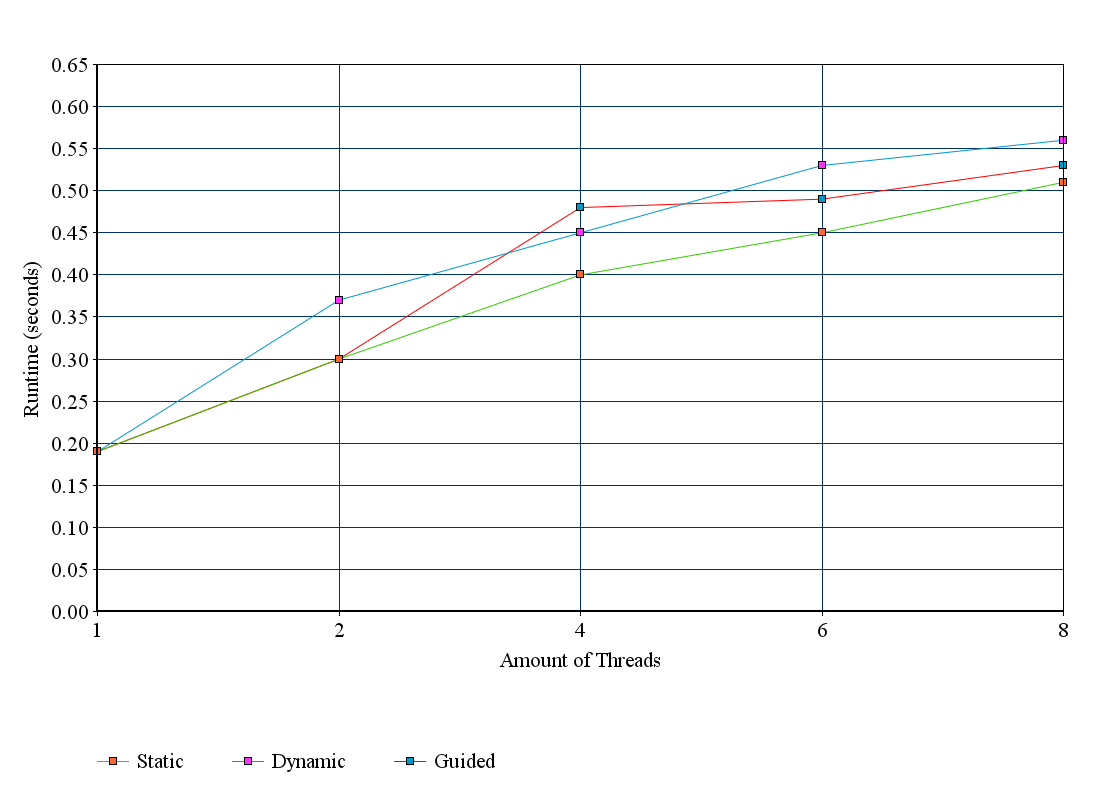
\includegraphics[width=\textwidth]{1000}
    \caption{Runtime of matrix generation and summing. Generates and sums 100
    matrices of size 1000x1000. Comparing Static, Guided and Dynamic (chunk size
    = 4 * matrix width / number of threads) scheduling.}
\end{figure}

\begin{figure}[H]
    \centering
    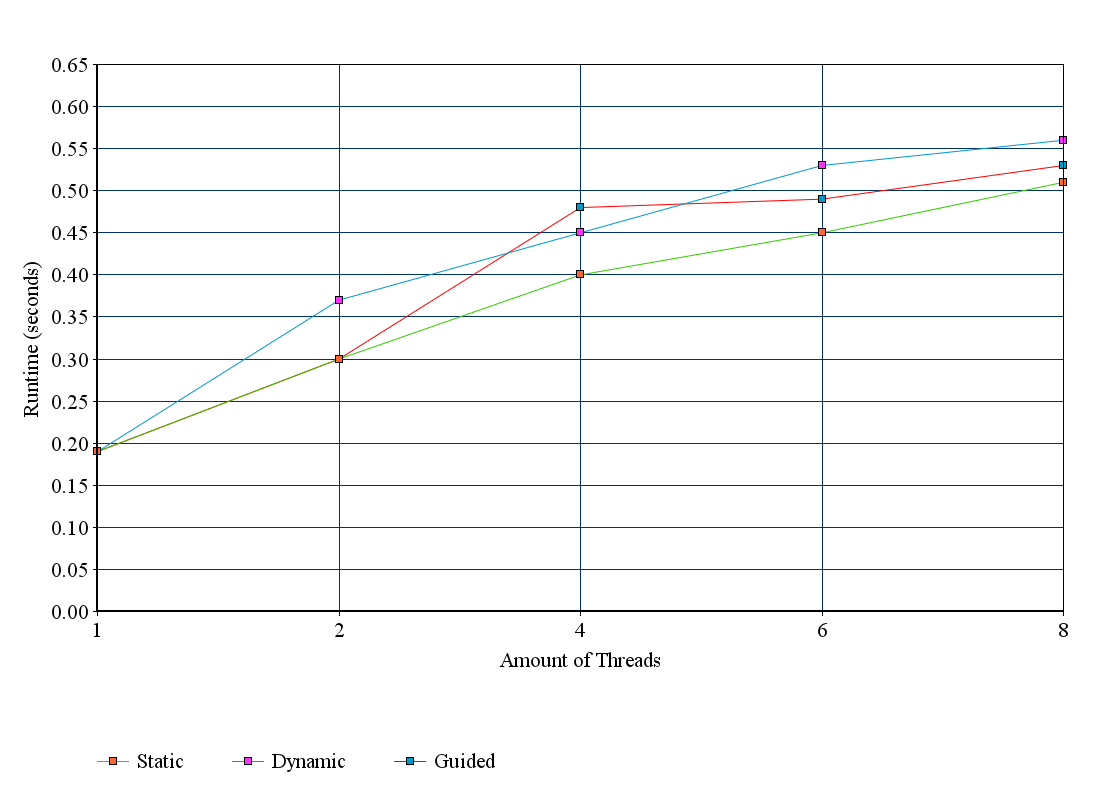
\includegraphics[width=\textwidth]{1000}
    \caption{Runtime of matrix generation and summing. Generates and sums 100
    matrices of size 5000x5000. Comparing Static, Guided and Dynamic (chunk size
    = 4 * matrix width / number of threads) scheduling.}
\end{figure}

\section{Discussion}
As stated above, parallelising this program using OpenMP did not have a great
effect. The program actually got slower the more threads we used. This is most
likely caused by overhead that is created by the creating and synchronising of
threads by OpenMP. This was not at all what we expected to happen, since this
program looks like a program that should be good for parallelising, as it is
doing matrix operations. So we were surprised to find that the overhead that is
caused is greater the actual benefit of parallelisation.



% =================================== REFERENCES ===================================

%\clearpage
%\bibliographystyle{unsrt}
%\bibliography{bib}

\end{document}
